% Preamble
% ---
\documentclass{article}

% Packages

\usepackage{graphicx}
\usepackage{subfig}

% ---


\graphicspath{ {assets/} }
\begin{document}


\section{Ground Truth}

Limitation of TPR. Difficult to define "true" values. The bouding region of a
face is discrete and we may choose not to detect side on faces. Example below
shows 2 possible "true" values for a detection. One give a IOU of under 0.7 but
the other gives over 0.9.

% -- Part 1 - Image section
\begin{figure}
\begin{tabular}{cccc}
\subfloat[dart4]{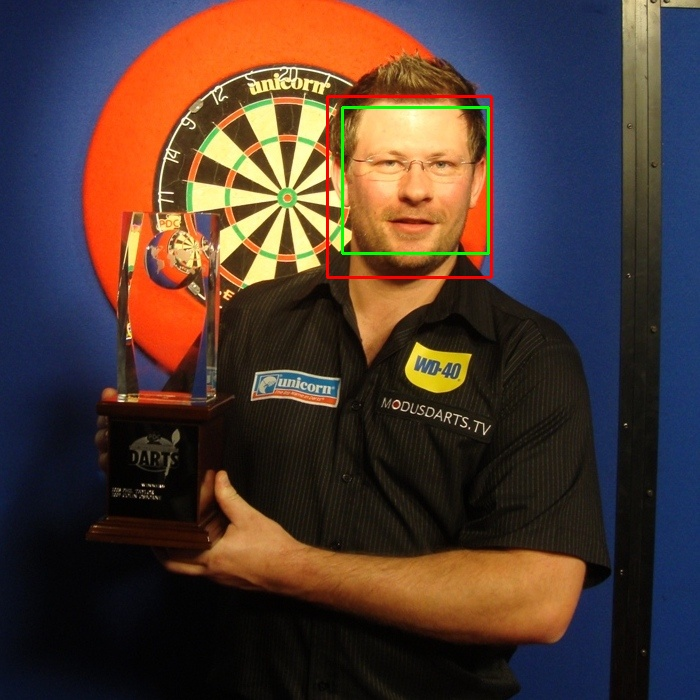
\includegraphics[width = 1.4in]{dart4-face}} &
\subfloat[dart5]{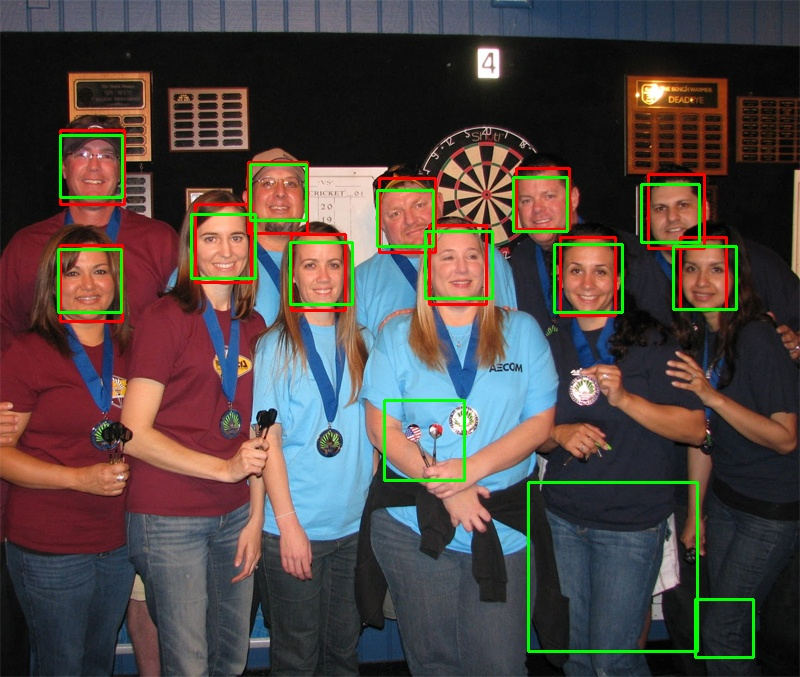
\includegraphics[width = 1.4in]{dart5-face}} &
\subfloat[dart13]{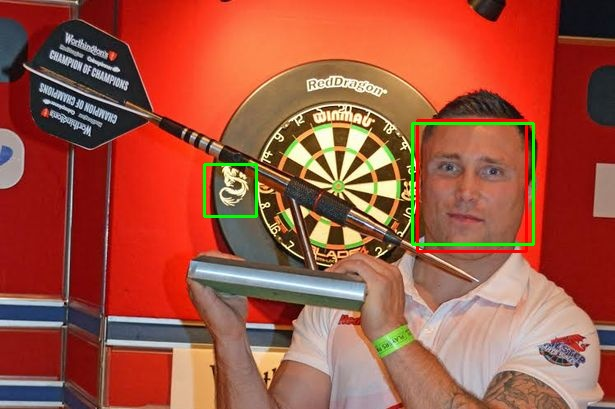
\includegraphics[width = 1.4in]{dart13-face}} \\
\subfloat[dart14]{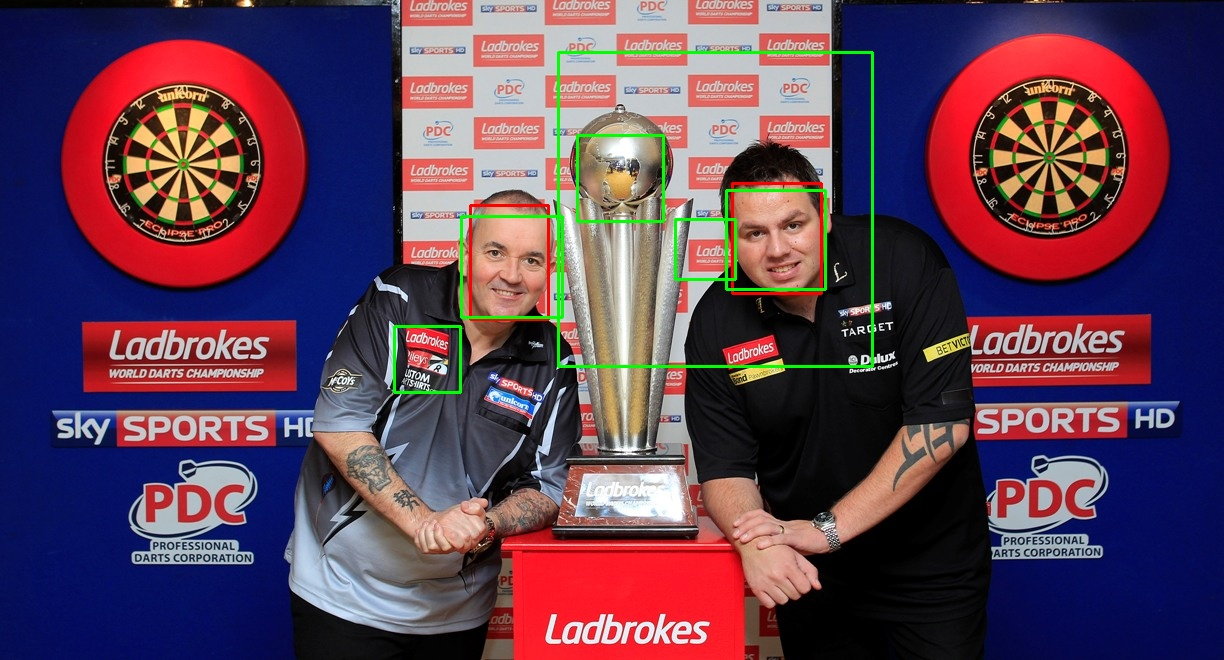
\includegraphics[width = 1.4in]{dart14-face}} &
\subfloat[dart15]{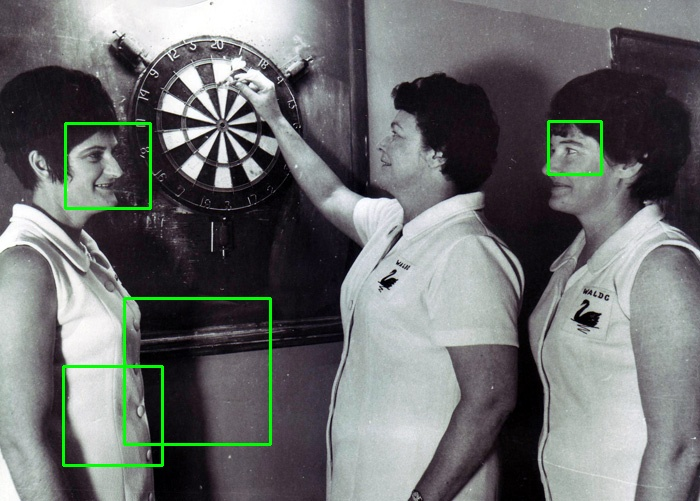
\includegraphics[width = 1.4in]{dart15-face}} &
\end{tabular}
\caption{Frontal face detection with ground truth}
\end{figure}


\begin{tabular}{ |p{3cm}||p{3cm}|p{3cm}| }
 \hline
 \multicolumn{3}{|c|}{Frontal face detection results} \\
 \hline
 Image name & TPR & F1-SCORE \\
 \hline
 dart4  & 1   & 1         \\
 dart5  & 1   & 0.88      \\
 dart13 & 1   & 0.666667  \\ 
 dart14 & 1   & 0.5       \\ 
 dart15 & 1   & 0         \\ 
 \hline
\end{tabular}

\end{document}
